\section{Design Process or Methodology Overview }
CivicRAG separates offline corpus/index construction from online retrieval and answer generation. The pipeline diagram in Figure~\ref{fig:architecture} describes the selected-evidence configuration used by the main CivicRAG run. Legacy controlled-answer branches remain in the repository for rollback but are not the answer route of this comparison.

\begin{figure}[p]\centering
\begin{singlespace}
\begin{tikzpicture}[x=1cm,y=1cm]
\tikzset{civicbox/.append style={font=\footnotesize,inner sep=2mm}}
\fill[rounded corners=3mm,civicTeal!4] (-0.2,0.9) rectangle (14.2,-4.1);
\node[anchor=west,font=\small\bfseries,text=civicTeal] at (0,0.55) {OFFLINE: CORPUS AND INDEX PREPARATION};
\node[civicbox,text width=5.5cm] (raw) at (3.1,-0.45) {Source files + prepared text\\PDF / DOCX / HTML / JSON};
\node[civicbox,text width=5.5cm] (chunk) at (10.6,-0.45) {Normalize and create typed chunks\\Attach IDs and provenance};
\draw[civicarr] (raw)--(chunk);
\node[civicbox,text width=12.6cm] (represent) at (7,-1.85) {Linked representations per chunk: search text $r_i$ and evidence $e_i$\\Only $r_i$ is embedded; $e_i$ is preserved as source content};
\draw[civicarr] (chunk.south)--(represent.north -| chunk.south);
\node[civicbox,text width=12.6cm] (indexes) at (7,-3.2) {BGE-M3($r_i$) $\rightarrow$ Chroma dense index\quad |\quad BM25 tokens from $r_i$\\Evidence and metadata remain linked by the same chunk ID};
\draw[civicarr] (represent)--(indexes);

\fill[rounded corners=3mm,civicBlue!4] (-0.2,-4.5) rectangle (14.2,-16.95);
\node[anchor=west,font=\small\bfseries,text=civicBlue] at (0,-4.9) {ONLINE: SHARED THREE-DOMAIN QUESTION ANSWERING};
\node[civicbox,text width=11.6cm] (query) at (7,-5.8) {Bangla question + selected domain\\Birth/death registration / Passport / BRTA};
\node[civicbox,text width=5.3cm] (dense) at (3.3,-7.25) {Dense search: top 20\\BGE-M3 query vector + Chroma};
\node[civicbox,text width=5.3cm] (sparse) at (10.7,-7.25) {BM25 search: top 20\\Query tokens + sparse index};
\draw[civicarr] (query.south)--++(0,-0.25)-|(dense.north);
\draw[civicarr] (query.south)--++(0,-0.25)-|(sparse.north);
\draw[civicarr,dashed] (indexes.west)--(-0.05,-3.2)--(-0.05,-7.25)--(dense.west);
\draw[civicarr,dashed] (indexes.east)--(14.05,-3.2)--(14.05,-7.25)--(sparse.east);
\node[civicbox,text width=11.6cm] (rrf) at (7,-8.75) {Weighted RRF: merge ranks, retain up to 15 candidates};
\draw[civicarr] (dense.south)--++(0,-0.25)-|(rrf.north);
\draw[civicarr] (sparse.south)--++(0,-0.25)-|(rrf.north);
\node[civicbox,text width=11.6cm] (rank) at (7,-10.0) {BGE cross-encoder reranking: ALL domains\\Lexical fallback if the cross-encoder is unavailable};
\draw[civicarr] (rrf)--(rank);
\node[civicbox,draw=civicGold,fill=civicGold!8,text width=11.6cm] (rules) at (7,-11.5) {Conditional birth-registration rules only:\\score adjustments and correction-fee supplementation\\Passport / BRTA skip these extra rules, not reranking};
\draw[civicarr] (rank)--(rules);
\node[civicbox,text width=11.6cm] (select) at (7,-13.1) {Shared applicability selector + compatible-family ordering\\Original evidence by ID; at most 6 chunks / 14,000 characters};
\draw[civicarr] (rules)--(select);
\node[civicbox,text width=11.6cm] (llm) at (7,-14.6) {Qwen3:8b: question + selected source evidence\\No evidence: clarification instead of an LLM answer};
\draw[civicarr] (select)--(llm);
\node[civicbox,text width=11.6cm] (answer) at (7,-16.1) {Bangla response + supplied source IDs\\Language check and incomplete-output warning};
\draw[civicarr] (llm)--(answer);
\end{tikzpicture}
\end{singlespace}
\caption{Earlier compact CivicRAG architecture with offline/online organization for three domains. Dashed arrows indicate index access. The gold box distinguishes domain-specific rules from shared reranking. The selected-evidence route bypasses the legacy controlled-answer branch.}\label{fig:architecture}
\end{figure}


The diagram retains the P2 separation between offline preparation and online answering, but explicitly connects stored evidence to generation and distinguishes shared components from conditional rules. The upper stage constructs retrieval resources; it is indexing, not LLM training. The lower stage searches and selects evidence before generating text. Dense retrieval, BM25, rank fusion, cross-encoder reranking, applicability selection and local generation are shared across all three configured domains. Only the additional registration-specific adjustments are conditional on the birth/death domain.

\section{Preliminary Design or Design (Model) Specification}
The P2 design emphasized birth/death registration, hybrid retrieval and controlled answer paths. Later work extended the corpus to passport and BRTA, added applicability selection and changed the main generator comparison to Qwen3. The final reported route therefore differs from the old diagrams that send every answer through a generic safe-path box.

The system is not an autonomous agent that performs government actions. Its task is single-turn retrieval and evidence-conditioned text generation. A domain is selected before retrieval. A targeted cross-domain aggregate guard handles certain multi-service questions, but comprehensive intent recognition is not claimed. Neither the lexical rules nor the selector is a separately trained classifier.

The implemented alternatives are the matched dense-only baseline and the design using hybrid retrieval, reranking and selected evidence. Both have saved 30-question executions. The relevant-only and evidence-order diagnostics isolate context handling but do not simulate a complete deployment. Their outputs verify specific design behaviours; a selector-off ablation remains unexecuted. Controlled settings appear in Section 4.4 and observed outcomes in Chapter 5.

\pending{Task DS-01: if component-level verification is required, freeze both configurations and run a selector-off comparison on the same questions, saving contexts, answers, timings and routes. Do not describe it as completed before its artifacts exist. The existing paired design comparison can be reported without inventing a simulation.}

\section{Data Collection -(If
Applicable)}
\paragraph{Needs-Analysis Questionnaire.}
The team supplied three CSV questionnaire exports, each containing 46 columns. They cover demographics, experiences with birth registration, passport and BRTA services, and a common nine-item block concerning a prospective AI assistant. The three versions place the service-specific blocks in different orders. Analysis aligns those blocks before checking identical submissions and uses column positions because several free-response headers repeat. The survey is a requirements input, not additional retrieval evidence, and is not ingested into the chatbot's knowledge base.

Only affirmative-consent records with a declared adult age group enter the main descriptive analysis. This conservative inclusion rule was applied when preparing the thesis analysis; it is not claimed to have been preregistered. Missing responses are excluded separately for each item, not interpreted as rejection. Percentages are computed as $100c/n_v$, where $c$ is the number selecting a response and $n_v$ the number answering that item. Multiple-selection items count each explicitly selected option once per submission, so their percentages need not sum to 100. A free-text ``all options'' response is retained in the denominator but not expanded into checked options. Open-text answers are not quoted publicly or automatically coded as validated themes.

The exported consent field establishes an affirmative response, not independent ethics approval. Recruitment method, invitation count, repeat-participation controls and consent arrangements for minors were not supplied. Accordingly, a response rate and nationally representative estimates cannot be calculated. The BRTA website question also combines a Bangladesh address with \code{rsta.gov.bt}; that item is not used to claim verified BRTA website usage. The main findings use the identically positioned common AI block and are reported in Chapter 5.

\paragraph{Source Families and Original Preservation.}
The birth/death collection contains structured JSON and prepared Markdown derived from FAQs, laws, rules, fees, correction processes and application guidance. Passport and BRTA were supplied as original-file directories and separately prepared Markdown. Passport derivatives are registered from \code{cleaned_md}; BRTA derivatives from \code{brta} and \code{fahim_brta}. Directories explicitly marked original are reference materials, not duplicate text automatically added to the answer corpus.

The register preserves document IDs, relative paths, snapshots, hashes, candidate original-file matches, inclusion history and chunk IDs. Candidate original matches do not certify textual fidelity. Some matches remain unresolved and are flagged. The distinction between collected originals and derivatives avoids counting the same information twice as independent evidence.

The corpus is a retrieval resource, not a newly annotated gold-answer benchmark. Its novelty is the organization of selected civic-service material into a source-traceable, machine-usable representation spanning the three domains. It is neither a census of all government documents nor a guarantee of current legal validity.

\subsection{Data Cleaning}
\begin{figure}[htbp]\centering
\begin{singlespace}
\begin{tikzpicture}[node distance=7mm]
\node[civicbox,text width=12.3cm] (original) {Collected originals + team-prepared derivatives\\Preserve originals; record the source relationship};
\node[civicbox,text width=12.3cm,below=of original] (parse) {Parse Markdown / structured JSON; read available front matter\\Normalize Unicode NFC and remove selected authoring artifacts};
\node[civicbox,text width=12.3cm,below=of parse] (split) {Document-type / heading-aware chunking\\Preserve FAQ pairs, fee conditions and procedure sections where available};
\node[civicbox,text width=12.3cm,below=of split] (meta) {Attach chunk IDs, document types, headings, source paths and available URLs\\Retain unresolved provenance / OCR / applicability flags};
\node[civicbox,text width=12.3cm,below=of meta] (output) {Domain JSONL: $(\mathrm{id}_i,r_i,e_i,m_i)$\\Build indexes from the configured active corpus};
\foreach \a/\b in {original/parse,parse/split,split/meta,meta/output}{\draw[civicarr] (\a)--(\b);}
\end{tikzpicture}
\end{singlespace}
\caption{Source-preserving preparation of the active corpus: original materials remain available while normalized derivatives are organized into identifiable retrieval units. Separate cleanup candidates are not substituted for the evaluated corpus.}\label{fig:preprocessing}
\end{figure}

Figure~\ref{fig:preprocessing} separates preservation of original materials from transformations applied to the machine-readable derivatives. The archived P2 diagram is a design reference; this final diagram describes supported preparation steps rather than assuming every originally illustrated operation was automated.

The active passport/BRTA ingestion parses simple front matter, normalizes NFC text, removes explicit authoring citation markers and selected invisible characters, and tracks headings. It preserves malformed or unrecognized material instead of making broad deletions. The work does not substantiate a universal automatic OCR repair or Bijoy-to-Unicode conversion stage for every supplied file; such claims from illustrative diagrams are not carried forward.

Separate cleanup candidates remove recognized authoring preambles and boilerplate and preserve larger structural units. Their manifests record changes and review flags. Those candidates must be distinguished from the evaluated corpus. At the audited snapshot, the active domain configurations still reference the heading-aware v2 passport/BRTA files. A later cleanup directory alone is not evidence that its contents were activated in ChromaDB or used in the saved answers.

\subsection{Data Transformation}
Document-type-aware transformation retains question-answer pairs, headings, fee rows and process sections where the source permits. A chunk should keep its governing condition with its answer. Splitting a heading from its body can make retrieval apparently relevant while the actual content answers a different question. Heading-aware ingestion was introduced to reduce this failure, but long unstructured legal OCR remains difficult.

Each chunk has the form
\begin{equation}
c_i=(\mathrm{id}_i,r_i,e_i,m_i),
\end{equation}
where $e_i$ is evidence content, $r_i$ is search text and $m_i$ is metadata. Search text may include aliases or section descriptors. These additions help search; they are not source facts and are not meant to become answer evidence. No query-specific reference answer is inserted into the generator merely because it resembles a test question.

\subsection{Data Integration}
\begin{figure}[htbp]\centering
\begin{singlespace}
\begin{tikzpicture}[x=1cm,y=1cm]
\tikzset{civicbox/.append style={font=\footnotesize,inner sep=2mm}}
\node[civicbox,text width=12cm] (record) at (7,0) {One chunk record: $c_i=(\mathrm{id}_i,r_i,e_i,m_i)$};
\node[civicbox,text width=3.5cm] (search) at (2.1,-1.7) {Search text $r_i$\\Aliases / search wording};
\node[civicbox,text width=3.5cm] (evidence) at (7,-1.7) {Evidence $e_i$\\Original source content};
\node[civicbox,text width=3.5cm] (metadata) at (11.9,-1.7) {Metadata $m_i$\\Type, heading, source};
\draw[civicarr] (record.south)--++(0,-0.25)-|(search.north);
\draw[civicarr] (record)--(evidence);
\draw[civicarr] (record.south)--++(0,-0.25)-|(metadata.north);
\node[civicbox,text width=3.5cm] (embed) at (2.1,-3.4) {BGE-M3 encoder\\Dense vector $v_i$};
\draw[civicarr] (search)--(embed);
\node[civicbox,text width=12cm] (storage) at (7,-5.05) {Chroma record: ID + vector $v_i$ + document $e_i$ + metadata $m_i$\\Active JSONL also retains the complete chunk record};
\draw[civicarr] (embed.south)--++(0,-0.3)-|(storage.north);
\draw[civicarr] (evidence)--(storage);
\draw[civicarr] (metadata.south)--++(0,-1.1)-|(storage.north east);
\node[civicbox,text width=12cm] (fetch) at (7,-6.7) {Dense search returns matching IDs\\Runtime looks up those IDs in the active JSONL chunk map};
\draw[civicarr] (storage)--(fetch);
\node[civicbox,text width=12cm] (generation) at (7,-8.35) {Selector retains applicable evidence $e_i$\\LLM receives the question and text, not vector coordinates};
\draw[civicarr] (fetch)--(generation);
\end{tikzpicture}
\end{singlespace}
\caption{How answer evidence remains connected to a vector without being generated by the database. BM25 is a separate index of $r_i$, omitted here to isolate the dense-storage link. All arrows entering storage denote stored fields, not additional embeddings.}\label{fig:evidence-linkage}
\end{figure}

Each domain has its own configured JSONL corpus and Chroma collection. Metadata preserves service context and available source URLs. A stable chunk ID joins vector results back to the source record. The runtime dense retriever obtains IDs from Chroma and reconstructs retrieval results from the in-memory chunk map, making the active JSONL and index consistency essential.

In \code{scripts/build_index.py}, embeddings are computed from \code{retrieval_text}, whereas Chroma's \code{documents} contain \code{content}. The versioned ingestion script follows the same storage separation. Therefore answer evidence is stored alongside a vector; it is not itself an answer produced by Chroma. Chroma is a retrieval store, and the LLM produces the response only after evidence selection.

Figure~\ref{fig:evidence-linkage} makes this relationship explicit. If $I_q$ is a list of retrieved chunk IDs and $M$ is the active chunk map, then the corresponding evidence is obtained by
\begin{equation}
E_q=[M[i].\mathrm{content}:i\in I_q].
\end{equation}
This is an identifier lookup, not a comparison between a database-generated answer and a reference answer. The subsequent selector can remove candidates or append compatible family members; therefore the final supplied evidence need not equal the first retrieved list.

\subsection{Data Reduction }
Reduction is treated conservatively. FAQ duplicate handling and chunk boundaries can reduce repeated text, but semantic deduplication of the complete three-domain corpus has not been independently established. Original archives are retained. Passport and BRTA registers contain 30 and 132 derivative documents respectively; the active snapshot includes chunks from all of those registered derivatives. This statement does not imply that every original file has a resolved one-to-one derivative match.

\subsection{Summary of Preprocessed Data}
\begin{table}[htbp]\centering\small
\caption{Active corpus inventory computed from configured files. Source units are prepared documents, not independent facts.}
\begin{tabularx}{\linewidth}{Xrrr}\toprule
Domain & Source units & Registered originals & Chunks\\\midrule
Birth registration & 12 & Not comparable & 187\\
Passport & 30 & 27 & 361\\
BRTA & 132 & 133 & 3161\\
\bottomrule\end{tabularx}\end{table}

\begin{figure}[htbp]\centering
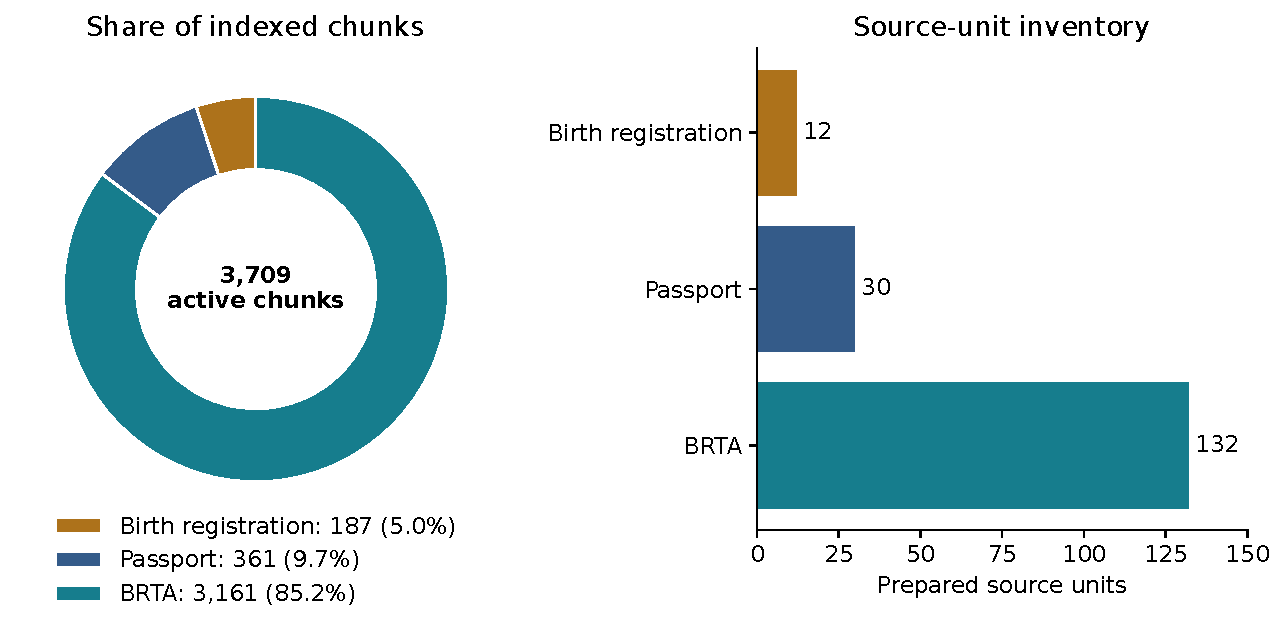
\includegraphics[width=\linewidth]{generated/corpus_distribution.pdf}
\caption{Active corpus composition from the frozen evidence manifest: 3,709 chunks and 174 prepared source units. Chunk share reflects document length and splitting, not demand, accuracy or unique facts.}\label{fig:corpus-distribution}
\end{figure}
Figure~\ref{fig:corpus-distribution} shows the corpus imbalance: BRTA accounts for 85.2\% of chunks, passport for 9.7\% and birth/death registration for 5.0\% (rounded independently). Domain-scoped retrieval prevents this corpus-size imbalance from directly mixing unrelated services in one query. It does not establish equal retrieval difficulty or equal source coverage across domains.
The table is computed from the configured JSONL files, not from unrelated candidate directories. For the older birth/death corpus, source units are counted using its source-path metadata. That count is not equated to a unique original-PDF count. Across domains, chunk counts are an indexing property rather than the number of independent facts or questions.

\begin{table}[htbp]\centering\small
\caption{Selected unresolved active-corpus flags, counted once per derivative document. These counts may overlap.}
\begin{tabularx}{\linewidth}{p{20mm}Xr}\toprule
Domain & Flag & Documents\\\midrule
Passport & no web address & 26\\
Passport & original match unresolved & 4\\
Passport & dated document review applicability & 1\\
Passport & long document check ocr & 0\\
BRTA & no web address & 109\\
BRTA & original match unresolved & 6\\
BRTA & dated document review applicability & 21\\
BRTA & long document check ocr & 8\\
\bottomrule\end{tabularx}\end{table}

Review flags count documents in the passport/BRTA registers or their associated chunk metadata, as indicated in the table. Multiple flags may apply to one document. A missing URL does not prove that a source is false, while a present URL does not prove that the derived text is correct. The flags identify where provenance and applicability need further review.

\section{Implementation of Selected Design}
\paragraph{Dense Embedding and Search.}
With encoder $f_\theta$, normalized vectors are
\begin{equation}
v_i=\frac{f_\theta(r_i)}{\|f_\theta(r_i)\|_2},\qquad
v_q=\frac{f_\theta(q)}{\|f_\theta(q)\|_2}.
\end{equation}
For unit vectors, squared Euclidean distance satisfies
\begin{equation}
\|v_q-v_i\|_2^2=2-2v_q^\top v_i.
\end{equation}
Thus distance and cosine induce the same exact ranking for normalized vectors. The index construction does not explicitly override Chroma's distance configuration; the thesis therefore does not assert that a cosine collection was manually configured. Approximate index search can differ from an exhaustive mathematical ranking.

BGE-M3 supplies the embedding model \cite{bgem3}; Chroma stores the vectors and linked documents \cite{chroma}. The implementation uses local cached model files and CPU embedding configuration. No corpus-specific gradient training occurs during this step.

\paragraph{BM25 Sparse Search.}
BM25 indexes tokens from $r_i$. Tokenization normalizes NFC, removes zero-width characters and extracts lower-case word/Bangla token sequences. The standard scoring structure is
\begin{equation}
\mathrm{BM25}(q,d)=\sum_{t\in q}\mathrm{IDF}(t)
\frac{f(t,d)(k_1+1)}{f(t,d)+k_1(1-b+b|d|/\overline L)}.
\end{equation}
Here $f(t,d)$ is term frequency, $|d|$ is token length and $\overline L$ is mean document length. The code instantiates \code{BM25Okapi} without explicit parameter overrides, so the installed library defaults determine $k_1$, $b$ and its IDF-floor behaviour \cite{bm25,rankbm25}. Lexical matching is a separate channel; it does not construct Chroma's vectors.

\paragraph{Weighted Reciprocal Rank Fusion.}
The implementation retrieves at most 20 candidates from each channel, omitting BM25 results with non-positive scores. It assigns one-based ranks and computes
\begin{equation}
S(d)=\frac{0.55\,\mathbf{1}[d\in D]}{50+r_D(d)}+
\frac{0.45\,\mathbf{1}[d\in B]}{50+r_B(d)}.
\end{equation}
A missing-channel term contributes zero. As an illustrative calculation, a chunk at dense rank 2 and BM25 rank 5 receives $0.55/52+0.45/55\approx0.01876$. This is a rank-combination value, not confidence in factual accuracy. The fused list is limited to 15 before reranking. The weights are implementation settings; this thesis does not claim they are optimal for the dataset.

\paragraph{Reranking and Domain-Specific Logic.}
The configured cross-encoder scores query/search-text pairs. If loading fails, the code can add a lexical-coverage adjustment of $0.05\,|T_q\cap T_d|/\max(|T_q|,1)$ to the incoming score. The saved primary CivicRAG candidate traces contain cross-encoder markers, establishing that the cross-encoder route was used in those records rather than merely being configured.

Birth/death-specific boosts and evidence augmentation remain part of the selected route. These are not universal learned mechanisms for passport and BRTA. This asymmetry should be disclosed when interpreting domain differences. An isolated ablation would be required to attribute an observed change to those rules.

\paragraph{Shared Reranking versus Registration-Specific Adjustments.}
The distinction is explicit in \code{src/pipeline.py}: \code{birth_death_rules} is true only for the \code{birth_death_registration} domain, and that flag is passed to the reranker's \code{domain_boosts} option. The cross-encoder itself is shared; passport and BRTA do not skip reranking. Its base score may be written as $s_{\mathrm{CE}}(q,r_i)=g_\phi(q,r_i)$, where the pretrained cross-encoder jointly processes the query and searchable passage. For a domain $d$, the implemented adjustment has the form
\begin{equation}
s_d(q,c_i)=s_{\mathrm{base}}(q,c_i)+
\mathbf{1}[d=\mathrm{birth/death}]\,\Delta_{\mathrm{registration}}(q,c_i).
\end{equation}
Here $s_{\mathrm{base}}$ is the cross-encoder score, or the documented fallback score when that model is unavailable. $\Delta_{\mathrm{registration}}$ is the sum of applicable hand-written adjustments, not a learned probability. For example, an application-process record receives an increment of 0.08 for a detected registration how-to query; additional heading conditions can further alter that score. These increments do not have a calibrated confidence interpretation.

Separately, \code{_augment_contexts} can append an existing correction-fee row for a detected date-of-birth or other data-correction query, provided its ID is not already present. It neither writes a new fact nor creates a synthetic answer. This registration-specific supplementation is different from the shared selector's compatible-family expansion, which can also operate on passport or BRTA evidence.

These rules reflect the earlier registration-focused implementation and its document-type schema. Applying the same conditions unchanged to other domains would be inappropriate: a birth-registration correction fee is not a passport or driving-licence correction fee. Equivalent domain rules were not implemented for passport and BRTA. This is an engineering asymmetry to disclose, not evidence that the extra rules are necessary or beneficial in every case. No pipeline change is made by documenting it.

\paragraph{Applicability Selection and Context Budget.}
The selector introduced after P2 uses service, action, product and location vocabularies. It prefers section scope over broad document titles and can reject a passport-collection passage for an application question. It also screens heading-only fragments, handles explicitly flagged historical alternatives and expands compatible fee/checklist families.

The selector is implemented in \code{src/generation/evidence_selection.py}; it is neither a second LLM nor a human choosing passages during normal operation. It retains at most six whole chunks within 14,000 characters. A chunk that does not fit is skipped rather than silently cut. A later ordering fix groups compatible family members near the first eligible anchor before applying the budget. Saved replay on 30 candidate sets changed the selected IDs for the passport-fee question while leaving the other 29 selections unchanged. This establishes the scope of that replay, not a general accuracy improvement.

For eligible candidates, the selector's initial priority is
\begin{equation}
h(q,c_i)=3A_i+S_i+2T_i,
\end{equation}
where $A_i$ indicates an overlapping action label, $S_i$ an overlapping service label and $T_i$ a fee/document-type match. Product, location and action conflicts can exclude a candidate before ordering. Ties retain the incoming candidate order. Historical-alternative filtering, checklist handling and compatible-family grouping are additional procedural steps, so this equation alone is not the entire selection algorithm.

For the resulting ordered list, the greedy whole-chunk selection obeys
\begin{equation}
|E|\leq 6,\qquad \sum_{c_i\in E}\operatorname{len}(e_i)\leq 14{,}000.
\end{equation}
The second bound uses Python string length in characters, not tokenizer tokens. This is a budget constraint, not a globally optimized evidence set. Skipping an oversized chunk can allow a later shorter chunk to enter the prompt.

An unknown or broad query can still retain unrelated material. Lexical applicability is not entailment, and a passage may contain mixed procedures even when its heading matches. The selector's decisions and expanded IDs are therefore retained in a trace. Removing the selector remains a proposed ablation, not a completed experiment in this manuscript.

\paragraph{Answer Generation and Safety Behaviour.}
Qwen3:8b receives the normalized question and selected evidence through Ollama \cite{qwen3,ollama}. The comparison uses temperature 0.05, top-$p$ 0.9, output limit 1,200 tokens, repetition penalty 1.18, repeat window 256 and selected-route context window 8,192. Qwen3 thinking is disabled. The prompt requests evidence-grounded Bangla responses and preservation of service conditions.

The current comparison bypasses legacy controlled extraction and question-category templates. If no applicable evidence remains, it returns a clarification/insufficient-information response. A heuristic language check can replace unsuitable-language output. A length finish reason produces an explicit incomplete-output warning. These are operational safeguards, not a complete factual verifier.

The answer's Sources footer identifies supplied context IDs, not verified supporting citations for each claim. The saved \code{raw_generation} field is produced after the generator's existing response canonicalization and should not be described as untouched token-level model output. Candidate sources and actual \code{answer_contexts} are stored separately to avoid evaluating unused passages as if the model had seen them.

\paragraph{Matched Simple RAG Baseline.}
The isolated runner \path{scripts/run_simple_matched.py} performs dense-only top-six retrieval. It does not call BM25 fusion, reranking, applicability selection, sibling expansion or controlled answers. It applies the same whole-chunk character budget, selected-route generation prompt, Qwen3 settings and language/truncation handling as the comparison configuration. The \code{selected_evidence=True} generator flag chooses the shared prompt; it does not invoke the selector inside the baseline.

\begin{table}[htbp]\centering\small
\caption{Controlled and varied elements of the main comparison.}
\begin{tabularx}{\linewidth}{p{44mm}XX}\toprule
Element & Simple RAG & CivicRAG\\\midrule
Corpus and questions & Same & Same\\
Generator and prompt & Qwen3, matched & Qwen3, matched\\
Dense retrieval & Top 6 & Top 20\\
BM25 and RRF & Absent & Present\\
Reranker & Absent & Present\\
Applicability/expansion & Absent & Present\\
Final context limit & 6 / 14,000 characters & 6 / 14,000 characters\\
Controlled answer bypass & Absent & Absent\\\bottomrule
\end{tabularx}\end{table}

The comparison intentionally keeps the baseline credible. It does not weaken the generator, restrict access to the corpus or remove successful baseline answers. It measures a bundled pipeline difference and cannot independently establish the benefit of every additional component.
